\documentclass{beamer}
\mode<presentation> {
    \usetheme{Copenhagen} \usecolortheme{whale}
    }
\usepackage{graphicx}
\usepackage{multicol}
\setbeamersize{text margin left=3mm,text margin right=5mm}

\graphicspath{{Images/}}

\title[Assignments 2]{Gradiente e DREM}
\author{Lorenzo Rossi Matricola: 0301285}
\begin{document}
\begin{frame}
	\titlepage{}
\end{frame}
\begin{frame}
	\begin{columns}[t]
		\begin{column}{.5\textwidth}
			\tableofcontents[sections={1-3}] % chktex 8
		\end{column}
		\begin{column}{.5\textwidth}
			\tableofcontents[sections={4-5}] % chktex 8
		\end{column}
	\end{columns}
\end{frame}
\begin{frame}
	\frametitle{Assignment 2}
	\section{Introduzione}
	Considerato il sistema:\begin{equation*}
		\dot{x}=-ax+bu,\quad a>0,b\neq{0}\:\text{non noti}
	\end{equation*}
	Determinare una parametrizzazione del sistema ed applicare gli identificatore dei parametri DREM e gradiente.
	Eseguire le simulazioni con \(a=0.4,b=0.4\) e i filtri per l'algoritmo DREM da utilizzare sono:
	\begin{equation*}
		H_{1}(s)=\frac{1}{s+1}\quad H_{2}(s)=\frac{2}{s+2}
	\end{equation*}
	Effettuare le simulazioni con \(u(t)=10\) e \(u(t)=10\sin{(\frac{5t}{2})}\) e valutare le performance dei due algoritmi.
\end{frame}
\begin{frame}
	\frametitle{Modello teorico}
	\section{Modello teorico}
	\begin{itemize}
		\item \textbf{Parametrizzazione lineare}:
		      \begin{tabular}{c}
			      $\begin{aligned}[t]
					       \dot{\phi_{1}} & =\Lambda_{c}\phi_{1}+\textit{l}u
					       \\
					       \dot{\phi_{2}} & =\Lambda_{c}\phi_{2}-\textit{l}y
					       \\
					       y              & =\theta_{1}^{T}\phi_{1}+ {(\theta_{2}-\lambda)}^{T}\phi_{2}
					       \\
					       z              & = y+\lambda^{T}\phi_{2}
				       \end{aligned}$
		      \end{tabular}
		\item \textbf{Gradiente}:
		\begin{tabular}{c}
			      $\begin{aligned}[t]
					       \dot{\hat{\theta}}=-\Gamma{(z-\hat{\theta}\phi)}\phi=\Gamma\phi\epsilon \\
					       \hat{z}=\theta^{T}\phi
				       \end{aligned}$
		\end{tabular}
		\item \textbf{DREM}:
		\begin{tabular}{c}
			$\begin{aligned}[t]
					 \mathcal{Z}& =\mathcal{H}z\quad\boldsymbol{\phi}=\mathcal{H}\phi^{T}\\
					 \tilde{\mathcal{Z}}&=adj\{\boldsymbol{\phi}\}\mathcal{Z}\quad\tilde{\mathcal{Z}}=\det{\{\boldsymbol{\phi}}\}\theta_{i}\\
					 \dot{\hat{\theta_{i}}}&=\gamma_{i}\det{\{\boldsymbol{\phi}\}} (\tilde{\mathcal{Z}}-\det{\{\boldsymbol{\phi}\}}\hat{\theta_{i}})
			\end{aligned}$
  \end{tabular}
	\end{itemize}
\end{frame}
\begin{frame}
	\frametitle{Simulink - 1}% chktex 8
\section{Implementazione Simulink}
\subsection{Parametrizzazione}
\begin{itemize}
	\item \textbf{Parametrizzazione Lineare}
\end{itemize}
	\begin{figure}
		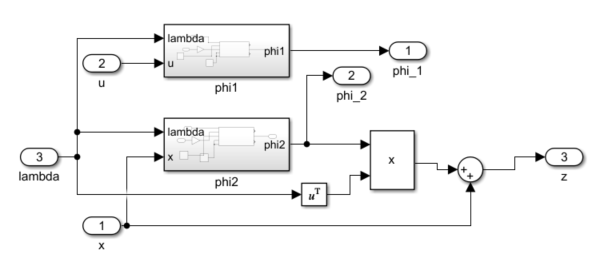
\includegraphics[scale=0.5]{2022-05-09-17-02-47.png} %chktex 8
	\end{figure}
\end{frame}
\begin{frame}
	\frametitle{Simulink - 2}% chktex 8
	\subsection{Gradiente}
	\begin{itemize}
		\item \textbf{Gradiente}
	\end{itemize}
	\begin{figure}
		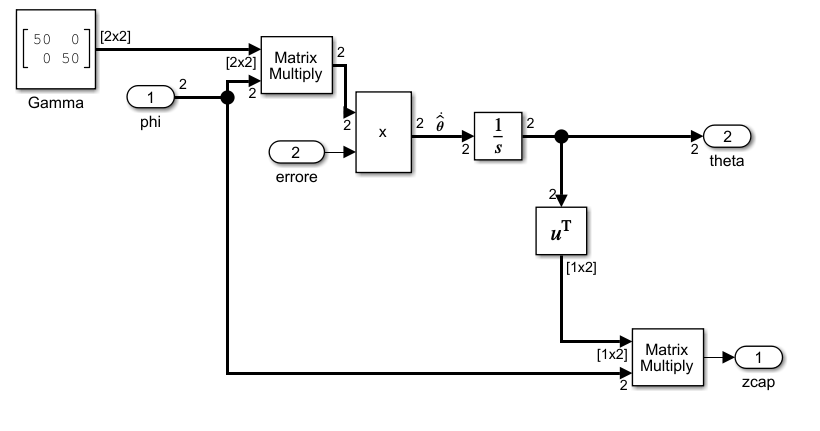
\includegraphics[scale=0.5]{2022-05-09-17-07-35.png}% chktex 8
	\end{figure}
\end{frame}
\begin{frame}
	\frametitle{Simulink -3}% chktex 8
	\subsection{DREM}
	\begin{itemize}
		\item \textbf{DREM}
	\end{itemize}
	\begin{figure}
		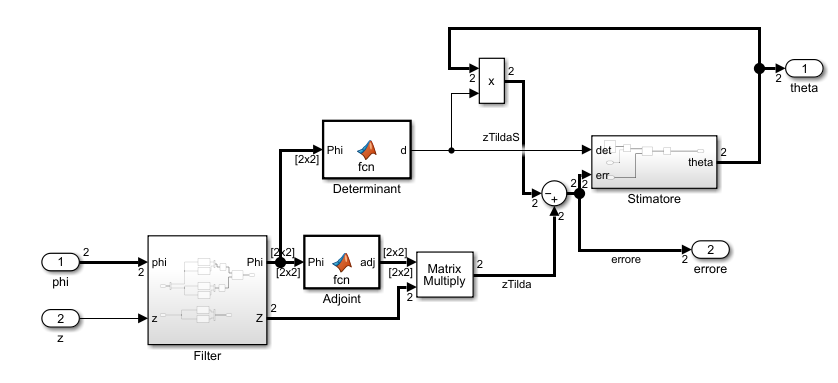
\includegraphics[scale=0.5]{2022-05-09-17-09-53.png} % chktex 8
	\end{figure}
\end{frame}
\begin{frame}
	\frametitle{Simulink - 4}% chktex 8
	\subsubsection{Filtro e Stimatore DREM}
	\begin{itemize}
		\item \textbf{Filtro}\begin{figure}
			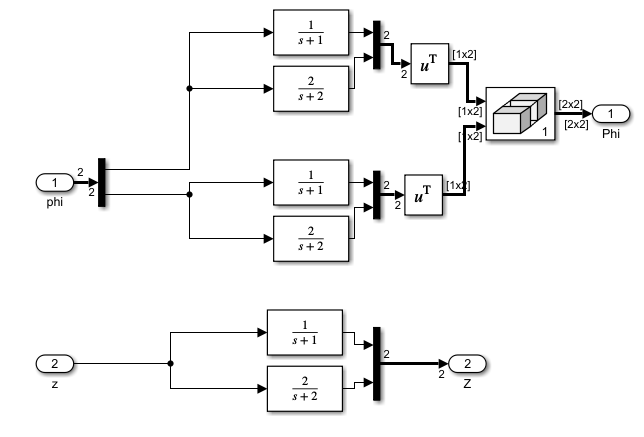
\includegraphics[scale=0.25]{2022-05-09-17-14-27.png}% chktex 8
		\end{figure}
		\item \textbf{Stimatore}\begin{figure}
			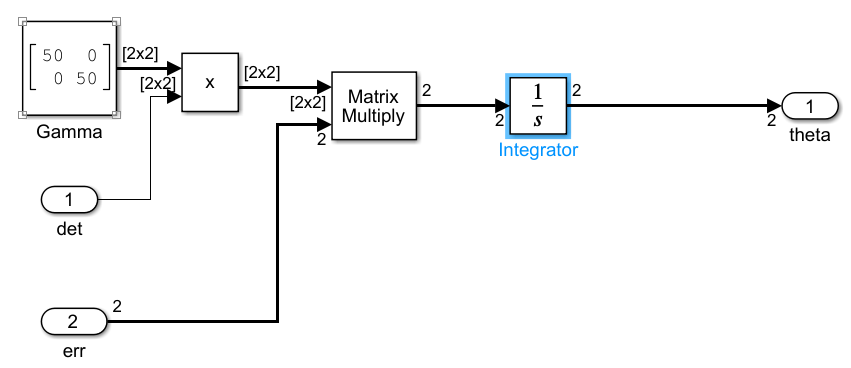
\includegraphics[scale=0.25]{2022-05-09-17-15-11.png}% chktex 8
		\end{figure}
	\end{itemize}
\end{frame}
\begin{frame}
	\frametitle{Simulink - 5}% chktex 8
	\subsection{Sistema complessivo}
	\begin{figure}
		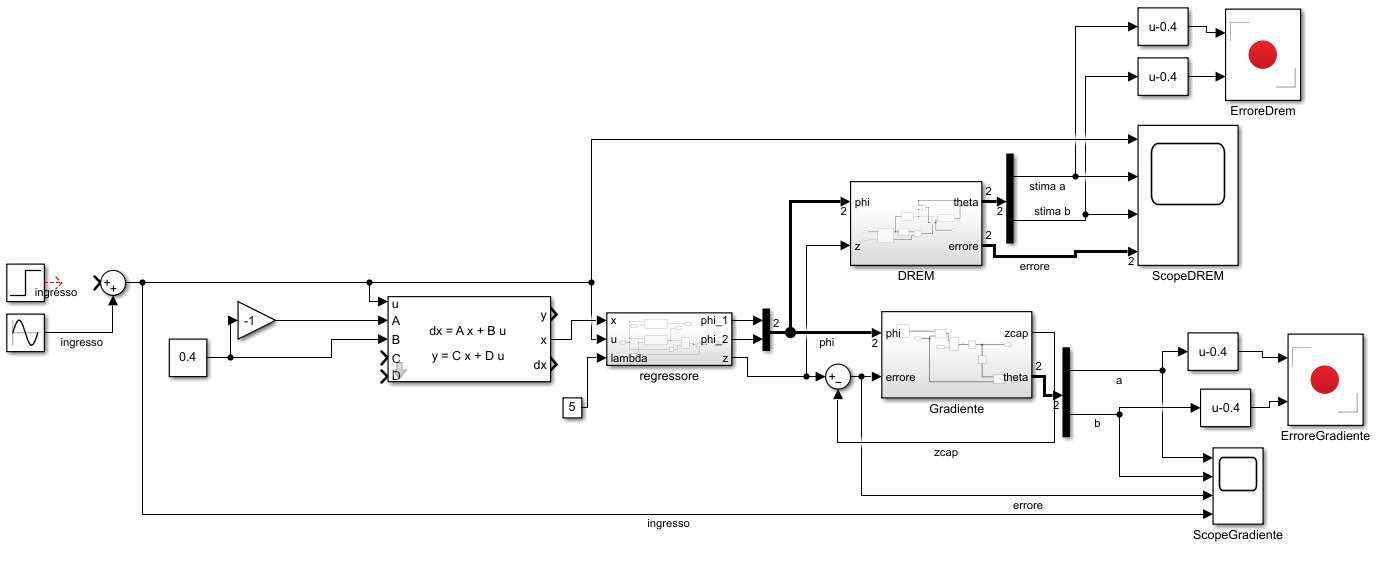
\includegraphics[scale=0.3]{2022-05-09-17-32-38.png} % chktex 8
	\end{figure}
\end{frame}
\begin{frame}
	\frametitle{Ingresso Gradino}
	\section{Analisi}
	\subsection{Ingresso gradino}
		\begin{minipage}[t]{0.42\textwidth}
			\textbf{Gradiente}
		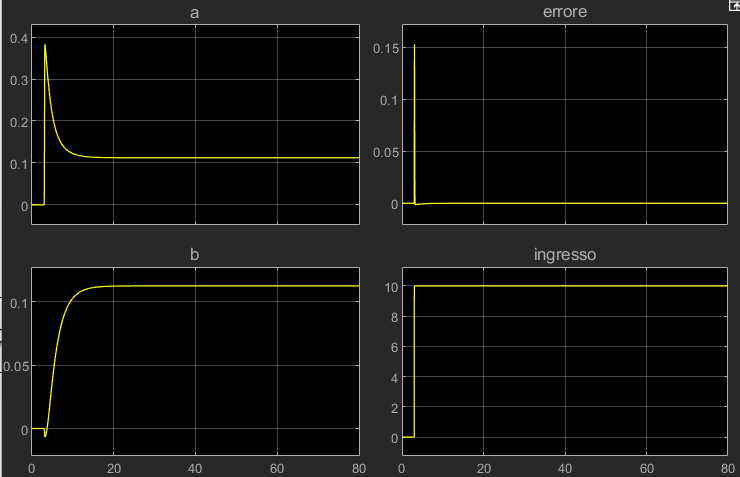
\includegraphics[scale=0.28]{2022-05-09-17-46-10.png}\newline% chktex 8
		\small
		L'errore converge a zero.Tuttavia, le stime dei parametri del sistema non convergono al valore vero dato che il segnale di ingresso è un segnale persistentemente eccitante ma non sufficientemente ricco.
	\end{minipage}\hspace{1cm}
	\begin{minipage}[t]{0.42\textwidth}
		\textbf{DREM}
		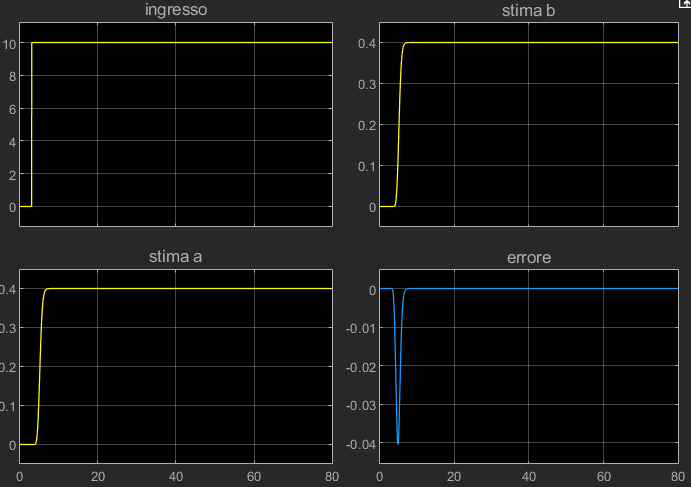
\includegraphics[scale=0.28]{2022-05-09-17-58-17.png} %chktex 8
		\small

		L'errore converge a zero in un tempo limitato ed assume valori più bassi rispetto a quelli ottenuti dall'algoritmo del gradiente. Inoltre, la stima dei parametri a e b converge al valore vero.
	\end{minipage}
\end{frame}
\begin{frame}
	\frametitle{Ingresso sinusoidale}
	\subsection{Ingresso Sinusoidale}
	\vspace{-0.1cm}
	\begin{minipage}[t]{0.42\textwidth}
		\textbf{Gradiente}
		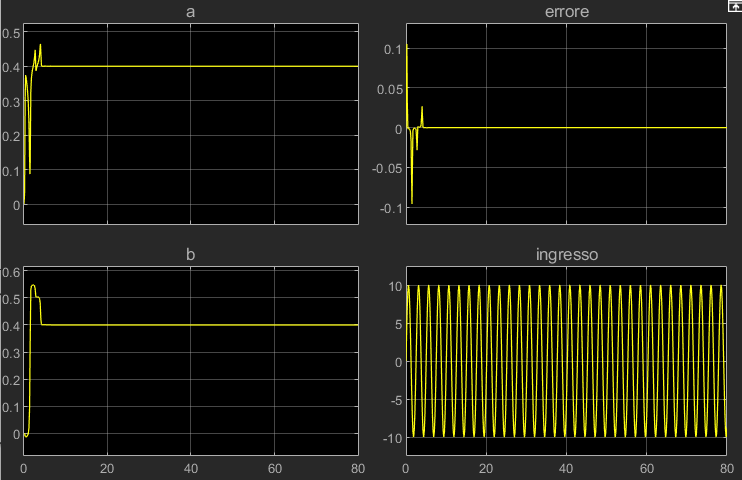
\includegraphics[scale=0.28]{2022-05-09-18-10-53.png}\\%chktex 8
		\footnotesize
				Il segnale è sufficientemente ricco e persistentemente eccitante quindi si ottiene la convergenza dell'errore e dei parametri. L'errore presenta delle oscillazioni durante il transitorio per poi arrivare a convergenza in circa 5-6 secondi.
	\end{minipage}\hspace{1cm}
	\begin{minipage}[t]{0.42\textwidth}
		\textbf{DREM}
		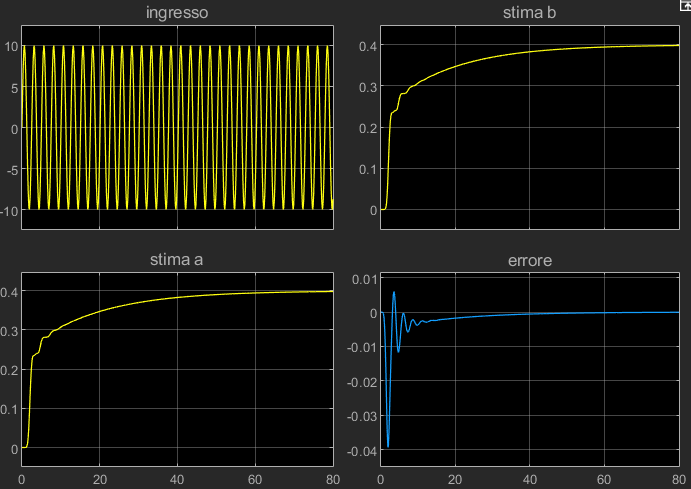
\includegraphics[scale=0.28]{2022-05-09-18-14-02.png}\\%chktex 8
		\footnotesize
		Anche nel DREM si ha la convergenza dell'errore e dei parametri, ma con un transitorio più lungo. Inoltre, l'andamento dei parametri è meno oscillatorio.Le sovraelongazioni sono dovute ai valori di \(\Gamma\) più o meno elevati come nel gradiente.
	\end{minipage}
\end{frame}
\begin{frame}
	\frametitle{Errore Stimatori}
	\subsection{Gradiente e DREM a confronto}
	\begin{minipage}[t]{0.45\textwidth}
		\textbf{Gradiente}
		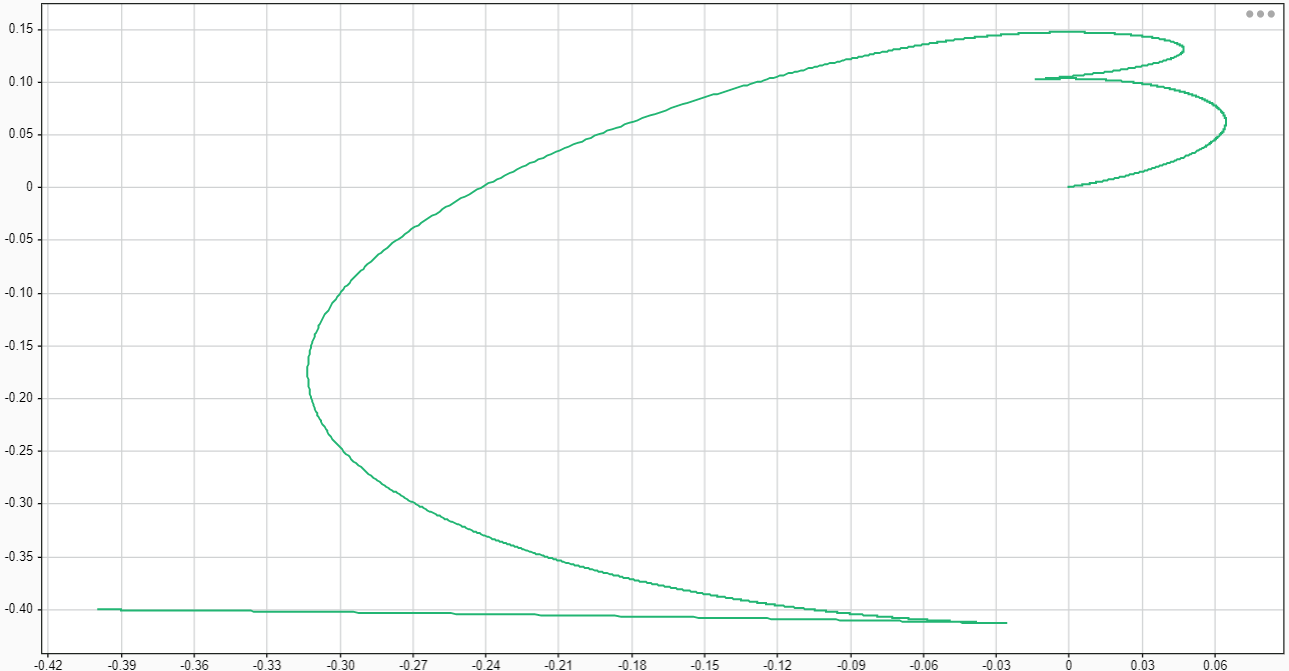
\includegraphics[scale=0.15]{2022-05-09-18-30-42.png}% chktex 8
	\end{minipage}\hspace{1cm}
	\begin{minipage}[t]{0.45\textwidth}
		\textbf{DREM}
		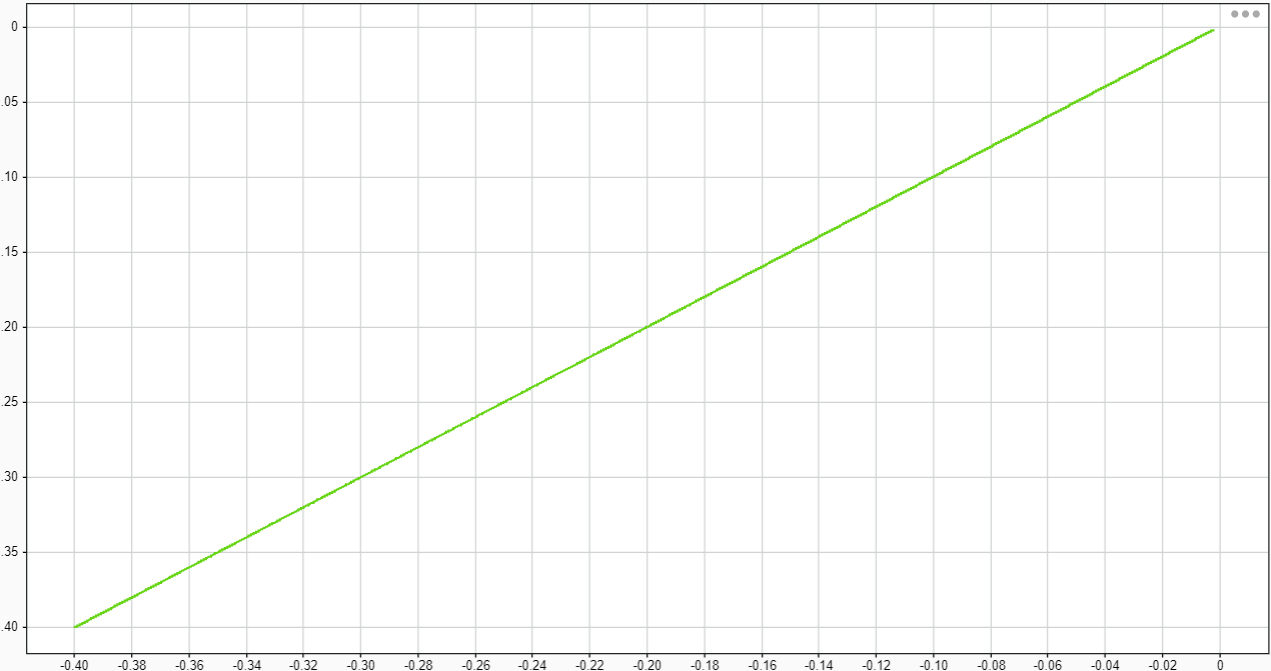
\includegraphics[scale=0.15]{2022-05-09-18-27-09.png}% chktex 8
	\end{minipage}
	La valutazione degli errori degli stimatori viene svolta con \(u=10\sin{(\frac{5t}{2})}\). In accordo con i grafici precedentemente mostrati, il gradiente dipende dalle condizioni operative in cui si trovano i parametri;mentre per il DREM si nota un andamento monotono decrescente. In particolare, entrambi gli algoritmi convergono a zero.
\end{frame}
\begin{frame}
	\frametitle{Conclusioni}
	\section{Conclusioni}
	Il modello DREM consente una stima dei parametri più lenta, ma con un transitorio più regolare e stime più precise a differenza del metodo del gradiente. Tuttavia, il metodo del gradiente presenza molte oscillazioni nel transitorio dovute alle condizioni in cui opera a vantaggio di un tempo di convergenza più veloce.
\end{frame}
\end{document}